% English dissertation follows Instructions on Project reports 22Feb16.pdf.
% Generated chapter files come from ../en/; edit those Markdown sources first.
\documentclass[a4paper,12pt,oneside,openany]{report}
\usepackage[left=25.4mm,right=20mm,top=20mm,bottom=20mm]{geometry}
\usepackage{setspace}
\usepackage[T1]{fontenc}
\usepackage{mathptmx}
\usepackage[scaled]{helvet}
\usepackage{courier,textcomp}
\usepackage[english]{babel}
\usepackage{amsmath,amssymb,booktabs,longtable,array,calc,graphicx,caption}
\usepackage{fvextra,xurl,etoolbox,needspace}
\usepackage[numbers,sort&compress]{natbib}
\usepackage[hidelinks,unicode]{hyperref}
\usepackage{bookmark}
% Personal fields remain explicit placeholders until supplied by the student.
\newcommand{\ThesisTitleEnglish}{Design and Implementation of a Multi-Agent Collaboration and Verification System for Code Repair}
\newcommand{\ThesisAuthor}{[Student name]}
\newcommand{\ThesisMatriculation}{[Matriculation number]}
\newcommand{\ThesisUESTCNumber}{[UESTC student number]}
\newcommand{\ThesisSupervisor}{[Supervisor name]}
\newcommand{\ThesisDegree}{BEng -- [Programme name]}
\newcommand{\ThesisAcademicYear}{[Academic year]}
\newcommand{\ThesisSubmissionDate}{[Submission date]}

\hypersetup{pdftitle={\ThesisTitleEnglish},pdfsubject={Final-year engineering dissertation}}
\setlength{\parindent}{1.5em}
\setlength{\parskip}{3pt}
\onehalfspacing
\setlength{\emergencystretch}{2em}
\clubpenalty=10000
\widowpenalty=10000
\setcounter{secnumdepth}{2}
\setcounter{tocdepth}{1}
\renewcommand{\thefigure}{\thechapter.\arabic{figure}}
\renewcommand{\thetable}{\thechapter.\arabic{table}}
\renewcommand{\theequation}{\thechapter.\arabic{equation}}
\newcounter{thesisalgorithm}[chapter]
\renewcommand{\thethesisalgorithm}{\thechapter.\arabic{thesisalgorithm}}
\captionsetup{labelsep=period,font=normalsize}
\captionsetup[table]{position=top}
\setlength{\LTleft}{\fill}
\setlength{\LTright}{\fill}
\AtBeginEnvironment{longtable}{\setlength{\tabcolsep}{4pt}\renewcommand{\arraystretch}{1.05}}
\DeclareUrlCommand\code{\urlstyle{tt}}
\providecommand{\tightlist}{\setlength{\itemsep}{0pt}\setlength{\parskip}{0pt}}
\setcounter{topnumber}{2}
\renewcommand{\topfraction}{0.9}
\renewcommand{\textfraction}{0.08}
\renewcommand{\floatpagefraction}{0.65}
\pagestyle{plain}
\usepackage{flafter}
\makeatletter
\newcommand{\ReportLayoutEvidence}{%
  \typeout{ReportFont=\f@size}%
  \typeout{ReportBaseline=\the\baselineskip}%
  \typeout{ReportPaperWidth=\the\paperwidth}%
  \typeout{ReportPaperHeight=\the\paperheight}%
  \typeout{ReportTextWidth=\the\textwidth}%
  \typeout{ReportTextHeight=\the\textheight}%
  \typeout{ReportLeft=\the\dimexpr1in+\oddsidemargin\relax}%
  \typeout{ReportTop=\the\dimexpr1in+\topmargin+\headheight+\headsep\relax}%
}
\makeatother

\begin{document}
\hypersetup{pageanchor=false}
\begin{titlepage}
  \centering
  \vspace*{18mm}
  {\Large School of Engineering\par}
  \vspace{3mm}
  {\Large University of Glasgow\par}
  \vspace{22mm}
  {\LARGE\bfseries \ThesisTitleEnglish\par}
  \vspace{16mm}
  {\large Final-Year Project Dissertation\par}
  \vfill
  \renewcommand{\arraystretch}{1.6}
  \begin{tabular}{@{}ll@{}}
    Student & \ThesisAuthor \\
    Matriculation number & \ThesisMatriculation \\
    UESTC student number & \ThesisUESTCNumber \\
    Supervisor & \ThesisSupervisor \\
    Degree programme & \ThesisDegree \\
    Academic year & \ThesisAcademicYear \\
    Submission date & \ThesisSubmissionDate
  \end{tabular}
  \vspace*{12mm}
\end{titlepage}
\pagenumbering{roman}
\hypersetup{pageanchor=true}
\chapter*{Abstract}
\addcontentsline{toc}{chapter}{Abstract}
% Generated from en/00-abstract.md; edit Markdown, then rebuild.
Coding agents can inspect repositories, edit source code and execute commands, but generating a plausible patch does not establish that a defect has been repaired. Repository-level repair also requires execution constraints, explicit acceptance criteria, failure feedback and resource control.

This dissertation presents a multi-agent collaboration and verification system built on an existing Python terminal coding agent. Coordinator, worker and verifier roles use separate contexts and sequential handoffs. Changes are made in disposable workspaces, commands execute in restricted Docker containers, and fixed acceptance tests run against a separate verification copy. Execution evidence supports bounded retries under shared budgets. The system exports patches and structured reports, with procedural skills and provenance-aware project memory integrated into the workflow.

Archived verification records report 160 passing automated tests, including existing regressions. Ten artificial defects were injected into pinned python-dotenv source: two development tasks and eight held-out tasks. Across 24 real model runs, single-role execution feedback, multi-role review feedback and multi-role verification feedback completed acceptance in eight, five and four cases respectively. No false acceptances were observed. Multi-role failures resulted from token-budget exhaustion; one additional candidate passed tests without completing its workflow.

Functional evidence supports the implemented isolation, acceptance, retry and reporting mechanisms. The small repair experiment does not demonstrate a success-rate advantage for multiple roles. Repair assessment must distinguish candidate behaviour from workflow completion and account for coordination costs.

\textbf{Keywords:} coding agent; multi-agent collaboration; code repair; execution evidence; resource budget.

\clearpage
\chapter*{Acknowledgements}
\addcontentsline{toc}{chapter}{Acknowledgements}
\noindent\textit{To be completed by the author.}
\clearpage
\begingroup
\setlength{\parskip}{0pt}
\tableofcontents
\endgroup
\clearpage
\listoffigures
\addcontentsline{toc}{chapter}{List of Figures}
\clearpage
\listoftables
\addcontentsline{toc}{chapter}{List of Tables}
\clearpage
\pagenumbering{arabic}
\ReportLayoutEvidence
% Generated from en/01-introduction.md; edit Markdown, then rebuild.
\chapter{Introduction}\label{chap:1}

\section{Background and motivation}\label{sec:1.1}

Repository repair requires a failure to be reproduced, relevant implementation to be located, a change to be made and regressions to be checked. A generated patch can look plausible while remaining incorrect. Likewise, a successful file write or a model's statement that a defect is fixed does not establish that the required behaviour has been restored.

Large language models (LLMs) can interact with repositories through tools. ReAct alternates reasoning, actions and observations; SWE-agent studies navigation, editing and execution through an agent-computer interface. These studies motivate an interactive coding workflow, but their results do not validate this implementation. \citep{yao2023react, yang2024sweagent}

Separate roles offer a way to divide planning, editing and inspection. AutoGen provides a reference for configurable conversational agents. Role separation also repeats information and consumes requests, so its value must be measured rather than assumed. \citep{wu2024autogen}

This dissertation extends the existing yeCoding Python terminal agent with a dedicated repair workflow. A coordinator organises the task, a worker edits a disposable copy and a verifier examines the candidate. Fixed tests, rather than review text, determine acceptance. Restricted execution and shared budgets constrain the process, while patches and structured records make successful and incomplete outcomes inspectable.

\section{Task definition and research questions}\label{sec:1.2}

A task comprises an issue description, current source state, prepared execution image, fixed acceptance commands and resource budgets. The output is a candidate patch with execution evidence and a termination state. The system does not automatically apply changes to the original repository.

Candidate behaviour and workflow completion are distinct. A candidate may pass tests while a subsequent required handoff exhausts the budget. Conversely, an already passing input does not establish that a repair occurred. These distinctions lead to three questions:

\begin{enumerate}
\def\labelenumi{\arabic{enumi}.}
\tightlist
\item
  \textbf{RQ1:} How can general coding capabilities be retained while bounding file changes and command execution, preserving original source and cleaning up after timeout or cancellation?
\item
  \textbf{RQ2:} How can role handoffs associate actual candidates with tests and reviews, supporting bounded retries without treating model assertions as acceptance?
\item
  \textbf{RQ3:} Under matched outer budgets, how do single-role execution feedback, multi-role review feedback and multi-role verification feedback differ in completion, consumption and failure categories?
\end{enumerate}

RQ3 permits adverse results for collaboration. The system targets Python tasks with runnable tests and caller-prepared environments. Model training, arbitrary-language semantics, concurrent patch merging and virtual-machine-level isolation are outside scope.

\section{Contributions and starting position}\label{sec:1.3}

The work builds on an existing agent rather than implementing all infrastructure from scratch. It contributes:

\begin{itemize}
\tightlist
\item
  A dedicated repair orchestrator with separate coordinator, worker and verifier histories, restricted tools and sequential handoffs.
\item
  Disposable editing and verification copies, candidate checks, restricted container commands and source-associated patch export.
\item
  Fixed acceptance, evidence-based feedback and shared attempt, request, token and time limits, with explicit unsuccessful states.
\item
  Integration of procedural skills and provenance-aware project memory.
\item
  Functional verification and a controlled comparison retaining failures and reporting candidate checks separately from completed workflows.
\end{itemize}

The command-line interface (CLI), interactive terminal, software development kit (SDK) and Runtime adapters reuse the same core. General ReAct, Plan and Team modes remain separate: repair-specific container and acceptance controls must not be attributed to every agent entry point. Skills and memory are functionally integrated, without an experimentally established independent quality benefit.

The dissertation proceeds from literature and specification to design, implementation, results, discussion and conclusions. Supporting details are in Appendix A; the central method and findings remain in the main text.

% Generated from en/02-related-technologies.md; edit Markdown, then rebuild.
\chapter{Literature Review and Technical Background}\label{chap:2}

\section{Repair models and fault localisation}\label{sec:2.1}

Automatic program repair separates a proposed change from the criterion used to accept it. Monperrus distinguishes repair objectives and oracles, while Gazzola et al.~survey generate-and-validate and semantics-driven approaches. These taxonomies motivate an explicit task definition: passing available tests establishes a bounded observation, not universal correctness. \citep{monperrus2018repair, gazzola2019survey}

GenProg searches program variants using genetic programming and existing tests. Nopol combines runtime observations and constraint solving for conditional bugs. Their generators and fault models differ, but both make the relationship between candidate search and executable constraints explicit. An LLM changes how candidates are proposed; it does not remove the need for an oracle. Neither study supplies a direct baseline for the present Python agent. \citep{legoues2012genprog, xuan2017nopol}

Fault localisation is a separate difficulty. Wong et al.~survey techniques for connecting observed failures to suspicious code. Here, lexical symbol retrieval helps navigation but is not spectrum-based localisation. Clear issue descriptions and local mutations reduce the localisation burden, limiting comparisons with unrestricted repository tasks. \citep{wong2016localization}

\section{Learned generation and richer evidence}\label{sec:2.2}

Tufano et al.~learn transformations from historical buggy/fixed code pairs. SequenceR uses sequence-to-sequence learning, selected context and a copy mechanism for one-line repair. These studies illustrate the relevance of source representation and candidate-generation constraints. Their developer-patch matches and supplied-location assumptions differ from behavioural repository acceptance; the present system neither trains these models nor reproduces their benchmarks. \citep{tufano2019neuralrepair, chen2021sequencer}

JAID uses state abstractions to extract information beyond ordinary tests for contract-based repair without supplied contracts. This provides a counterpoint to relying on test results alone, but a verifier reading logs does not implement JAID's semantic abstractions. Adding a review role cannot be described as equivalent semantic validation. \citep{chen2021contractrepair}

RepairLLaMA investigates repair-specific representations and parameter-efficient adaptation for Java bugs within one function. It offers a different route from orchestrating an unchanged model service: training and representation design, rather than role handoffs. The present system trains no adapters, and its Python workflow outcomes are not directly comparable to that evaluation. \citep{silva2025repairllama}

\section{Patch overfitting and assessment}\label{sec:2.3}

Yu et al.~distinguish regression introduction from incomplete fixing and examine generated tests for Nopol. Their findings indicate that extra tests can help without solving the oracle problem. This motivates protecting acceptance tests and distinguishing test adequacy from broader correctness. \citep{yu2019overfitting}

Ye et al.~assess patches at scale using generated tests and human repairs as reference oracles. Their QuixBugs study also examines plausible-patch correctness through manual and automatic assessment. These studies support checks beyond the suite that guided search, but their assessment techniques have assumptions and imperfections. The withheld tests here add evidence without reproducing those methods or proving correctness on untested inputs. \citep{ye2021assessment, ye2021quixbugs}

\section{Benchmarks and repository context}\label{sec:2.4}

ManyBugs and IntroClass establish documented C repair benchmarks for reproducible comparisons. SWE-bench instead connects real repository issues to executable evaluation. They motivate pinned inputs and clearly reported task construction. The injected python-dotenv defects used here are neither historical issues nor instances of these benchmarks; cross-benchmark success rates are not directly comparable. \citep{legoues2015manybugs, jimenez2024swebench}

RepoCoder combines repository retrieval with iterative completion. Lost in the Middle observes position-sensitive information use on its evaluated tasks. These results motivate selective context, without establishing a repair gain from this implementation's Python abstract syntax tree (AST) index. Its static relationships are approximate and its lexical retrieval does not use an embedding model. \citep{zhang2023repocoder, liu2024lostmiddle}

\section{Tool interaction and multiple roles}\label{sec:2.5}

ReAct and SWE-agent motivate observable repository tools and interaction design, as introduced in Chapter~\ref{chap:1}. AutoGen provides a reference for role organisation; Reflexion studies retaining textual feedback between attempts without updating model weights. Independent histories do not guarantee independent judgments when roles share a model and source. \citep{wu2024autogen, shinn2023reflexion}

Hou et al.'s systematic review spans model, data and evaluation choices in software engineering, reinforcing the need to qualify results by setting. Its search period does not represent a complete October 2026 state of the art. In this project, coordination cost is measured alongside acceptance rather than assumed beneficial. \citep{hou2024llmse}

Table~\ref{tab:2-1} synthesises the design implications and limits.

\begin{longtable}[]{@{}
  >{\raggedright\arraybackslash}p{(\linewidth - 6\tabcolsep) * \real{0.2200}}
  >{\raggedright\arraybackslash}p{(\linewidth - 6\tabcolsep) * \real{0.2400}}
  >{\raggedright\arraybackslash}p{(\linewidth - 6\tabcolsep) * \real{0.2500}}
  >{\raggedright\arraybackslash}p{(\linewidth - 6\tabcolsep) * \real{0.2900}}@{}}
\caption[Research findings and design implications]{Research strands informing the repair workflow and the limits on transferring their findings.}\label{tab:2-1}\tabularnewline
\toprule\noalign{}
\begin{minipage}[b]{\linewidth}\raggedright
Strand
\end{minipage} & \begin{minipage}[b]{\linewidth}\raggedright
Representative sources
\end{minipage} & \begin{minipage}[b]{\linewidth}\raggedright
Design implication
\end{minipage} & \begin{minipage}[b]{\linewidth}\raggedright
Limit
\end{minipage} \\
\midrule\noalign{}
\endfirsthead
\toprule\noalign{}
\begin{minipage}[b]{\linewidth}\raggedright
Strand
\end{minipage} & \begin{minipage}[b]{\linewidth}\raggedright
Representative sources
\end{minipage} & \begin{minipage}[b]{\linewidth}\raggedright
Design implication
\end{minipage} & \begin{minipage}[b]{\linewidth}\raggedright
Limit
\end{minipage} \\
\midrule\noalign{}
\endhead
\bottomrule\noalign{}
\endlastfoot
Repair/oracles & Surveys, GenProg, Nopol & Explicit acceptance and fault model & Tests are incomplete \\
Learned generation & Tufano, SequenceR & Selected source and bounded candidates & Different tasks/models \\
Assessment & Yu; Ye studies; JAID & Preserve independent evidence & Not a correctness proof \\
Benchmarks & ManyBugs; SWE-bench & Pin inputs and report provenance & Synthetic corpus is narrower \\
Context/agents & RepoCoder, ReAct, AutoGen & Tools, context and role contracts & Extra interaction costs resources \\
\end{longtable}

\section{Technical foundations}\label{sec:2.6}

The existing query loop can be represented by instructions \(I_t\), history \(H_t\), available tools \(\mathcal{T}_t\), model decision \(\pi_\theta\) and executor \(E\):

\begin{equation}
a_t=\pi_\theta(I_t,H_t,\mathcal{T}_t),\qquad
o_t=E(a_t),\qquad
H_{t+1}=H_t\oplus(a_t,o_t).\label{eq:2-1}
\end{equation}

This describes interaction, not model training. The executor validates actions and associates results by call identifier. A text response can end a role call without satisfying task acceptance.

Instructions, history, tools, evidence and output allowances compete for a context window \(W\):

\begin{equation}
B_{\mathrm{prompt}}+B_{\mathrm{history}}+B_{\mathrm{tools}}
+B_{\mathrm{evidence}}+B_{\mathrm{output}}+B_{\mathrm{reserve}}\leq W.\label{eq:2-2}
\end{equation}

Estimated tokens support code selection and conversation compression; provider usage measures consumption. Retrieval selects repository evidence, while history compression reduces past interaction. Skills supply reusable procedures; project memory supplies attributable experience. Neither grants permissions or overrides current tests.

Disposable copies protect original files, while host path checks restrict file tools. Container isolation uses host-kernel mechanisms such as namespaces, control groups and capabilities; sharing the kernel limits the separation it provides. These are configured constraints, not a universal security guarantee. \citep{sultan2019containers} The present runner's central processing unit (CPU), memory and command limits are implementation choices described in Chapter~\ref{chap:5} and checked by its functional tests.

% Generated from en/03-requirements-analysis.md; edit Markdown, then rebuild.
\chapter{Requirements and Specification}\label{chap:3}

\section{Tasks and scope}\label{sec:3.1}

The system serves terminal users, programmatic callers and evaluators. Each supplies an issue, current source directory, prepared container image, at least one fixed acceptance command and positive resource limits. Evidence is delivered outside the source workspace. Current file bytes establish the input: Git HEAD alone cannot identify uncommitted changes.

Dependencies must already exist in the image. Missing tests or an unavailable environment must produce explicit errors without host-shell fallback. Supported repair edits business source in disposable copies. Concurrent writers, automatic merges, binary patches, links, special files and tasks requiring protected-test changes are excluded.

\section{Functional specification}\label{sec:3.2}

Table~\ref{tab:3-2} defines the shared contracts. Different interfaces may organise parameters differently, but may not silently change acceptance semantics.

\begin{longtable}[]{@{}
  >{\raggedright\arraybackslash}p{(\linewidth - 4\tabcolsep) * \real{0.1400}}
  >{\raggedright\arraybackslash}p{(\linewidth - 4\tabcolsep) * \real{0.2700}}
  >{\raggedright\arraybackslash}p{(\linewidth - 4\tabcolsep) * \real{0.5900}}@{}}
\caption[Functional requirements]{Functional requirements for the repair workflow.}\label{tab:3-2}\tabularnewline
\toprule\noalign{}
\begin{minipage}[b]{\linewidth}\raggedright
ID
\end{minipage} & \begin{minipage}[b]{\linewidth}\raggedright
Requirement
\end{minipage} & \begin{minipage}[b]{\linewidth}\raggedright
Observable condition
\end{minipage} \\
\midrule\noalign{}
\endfirsthead
\toprule\noalign{}
\begin{minipage}[b]{\linewidth}\raggedright
ID
\end{minipage} & \begin{minipage}[b]{\linewidth}\raggedright
Requirement
\end{minipage} & \begin{minipage}[b]{\linewidth}\raggedright
Observable condition
\end{minipage} \\
\midrule\noalign{}
\endhead
\bottomrule\noalign{}
\endlastfoot
FR-01 & Repository tools & Read, search, edit and command results reflect execution; invalid inputs are rejected. \\
FR-02 & Code context & Retrieval retains source locations and identifies truncation. \\
FR-03 & Shared entry points & Core acceptance is consistent; unsuccessful outcomes are explicit. \\
FR-04 & Baseline & Source is recorded and a genuine failure established before repair. \\
FR-05 & Role handoffs & Separate histories and permitted tools refer to the same candidate. \\
FR-06 & Fixed acceptance & Real test results govern acceptance; protected checks cannot be weakened. \\
FR-07 & Bounded retry & Candidate-specific feedback and shared budgets control continuation. \\
FR-08 & Evidence delivery & Success exports a patch/report; failure retains available evidence. \\
FR-09 & Procedural skills & Actual role content, version and provenance are recorded. \\
FR-10 & Project memory & Scope, expiry and source applicability are checked. \\
\end{longtable}

A passing baseline does not count as a new repair. Worker summaries do not replace file differences; favourable reviews do not override failing tests. Empty changes or consecutive identical candidates end as no progress. A passing candidate is not a completed workflow if required handoffs remain unfinished.

Skills guide operations without granting permissions. Memory supplies untrusted historical leads, not current acceptance. Automatic successful experience is saved only after workflow success, with source and report provenance. Disabling memory skips recall and saving; recoverable storage problems produce warnings rather than overwrite established test facts.

\section{Non-functional specification}\label{sec:3.3}

Table~\ref{tab:3-3} separates execution constraints from quality claims. No minimum repair rate or universal collaboration benefit is specified.

\begin{longtable}[]{@{}
  >{\raggedright\arraybackslash}p{(\linewidth - 4\tabcolsep) * \real{0.1500}}
  >{\raggedright\arraybackslash}p{(\linewidth - 4\tabcolsep) * \real{0.2700}}
  >{\raggedright\arraybackslash}p{(\linewidth - 4\tabcolsep) * \real{0.5800}}@{}}
\caption[Non-functional requirements]{Non-functional requirements and their inspection conditions.}\label{tab:3-3}\tabularnewline
\toprule\noalign{}
\begin{minipage}[b]{\linewidth}\raggedright
ID
\end{minipage} & \begin{minipage}[b]{\linewidth}\raggedright
Requirement
\end{minipage} & \begin{minipage}[b]{\linewidth}\raggedright
Inspection condition
\end{minipage} \\
\midrule\noalign{}
\endfirsthead
\toprule\noalign{}
\begin{minipage}[b]{\linewidth}\raggedright
ID
\end{minipage} & \begin{minipage}[b]{\linewidth}\raggedright
Requirement
\end{minipage} & \begin{minipage}[b]{\linewidth}\raggedright
Inspection condition
\end{minipage} \\
\midrule\noalign{}
\endhead
\bottomrule\noalign{}
\endlastfoot
NFR-01 & Source/path boundaries & Copies contain edits; out-of-scope files and unsupported types are rejected. \\
NFR-02 & Resource limits & Commands/tasks have limits and cleanup on timeout or cancellation. \\
NFR-03 & Credential boundary & Model credentials are not forwarded; standard private-file patterns are excluded. \\
NFR-04 & Traceability & Candidate-linked evidence distinguishes success from incomplete execution. \\
NFR-05 & Integration consistency & Explicit options override configuration; cancelled tasks reject late completion. \\
NFR-06 & Evaluation clarity & Completion, additional checks and consumption use explicit all-run denominators. \\
\end{longtable}

Protection applies to supported file conventions, not arbitrary acceptance scripts or every possible secret. Containers restrict commands while host file tools require separate checks. Token usage is checked before a request, so a final response can cross the threshold. Cleanup may delay return beyond the nominal deadline; cancellation does not guarantee immediate interruption of a remote model request.

\section{Acceptance and evaluation}\label{sec:3.4}

Completion requires a genuine failing baseline, a non-empty legal candidate, passing fixed commands and delivery after all strategy-required stages. Functional scenarios cover missing commands, passing baselines, failed-then-passing retries, misleading positive reviews, boundary violations, no progress, exhausted budgets, unavailable images, timeout, cancellation and knowledge/interface integration. The detailed traceability matrix is in Table~\ref{tab:A-2}; the essential completion conditions remain specified here.

Comparative evaluation fixes source, model settings, environment, commands and outer limits. Development cases are excluded from the held-out denominator, and artificial defects are identified as such. Post-run checks assess exported patches without changing original termination states. Functional operation, repair quality and reproducibility are separate claims: records support inspection but cannot guarantee identical remote-model output.

% Generated from en/04-system-design.md; edit Markdown, then rebuild.
\chapter{System Design}\label{chap:4}

\section{Architecture and design choices}\label{sec:4.1}

Figure~\ref{fig:4-1} separates interfaces, orchestration, reusable capabilities and execution/storage. These are logical responsibilities in one application, not separate services. Interfaces collect options and display events; the orchestrator determines completion; the existing agent supplies model/tool interaction, context and knowledge.

\begin{figure}[htbp]
\centering
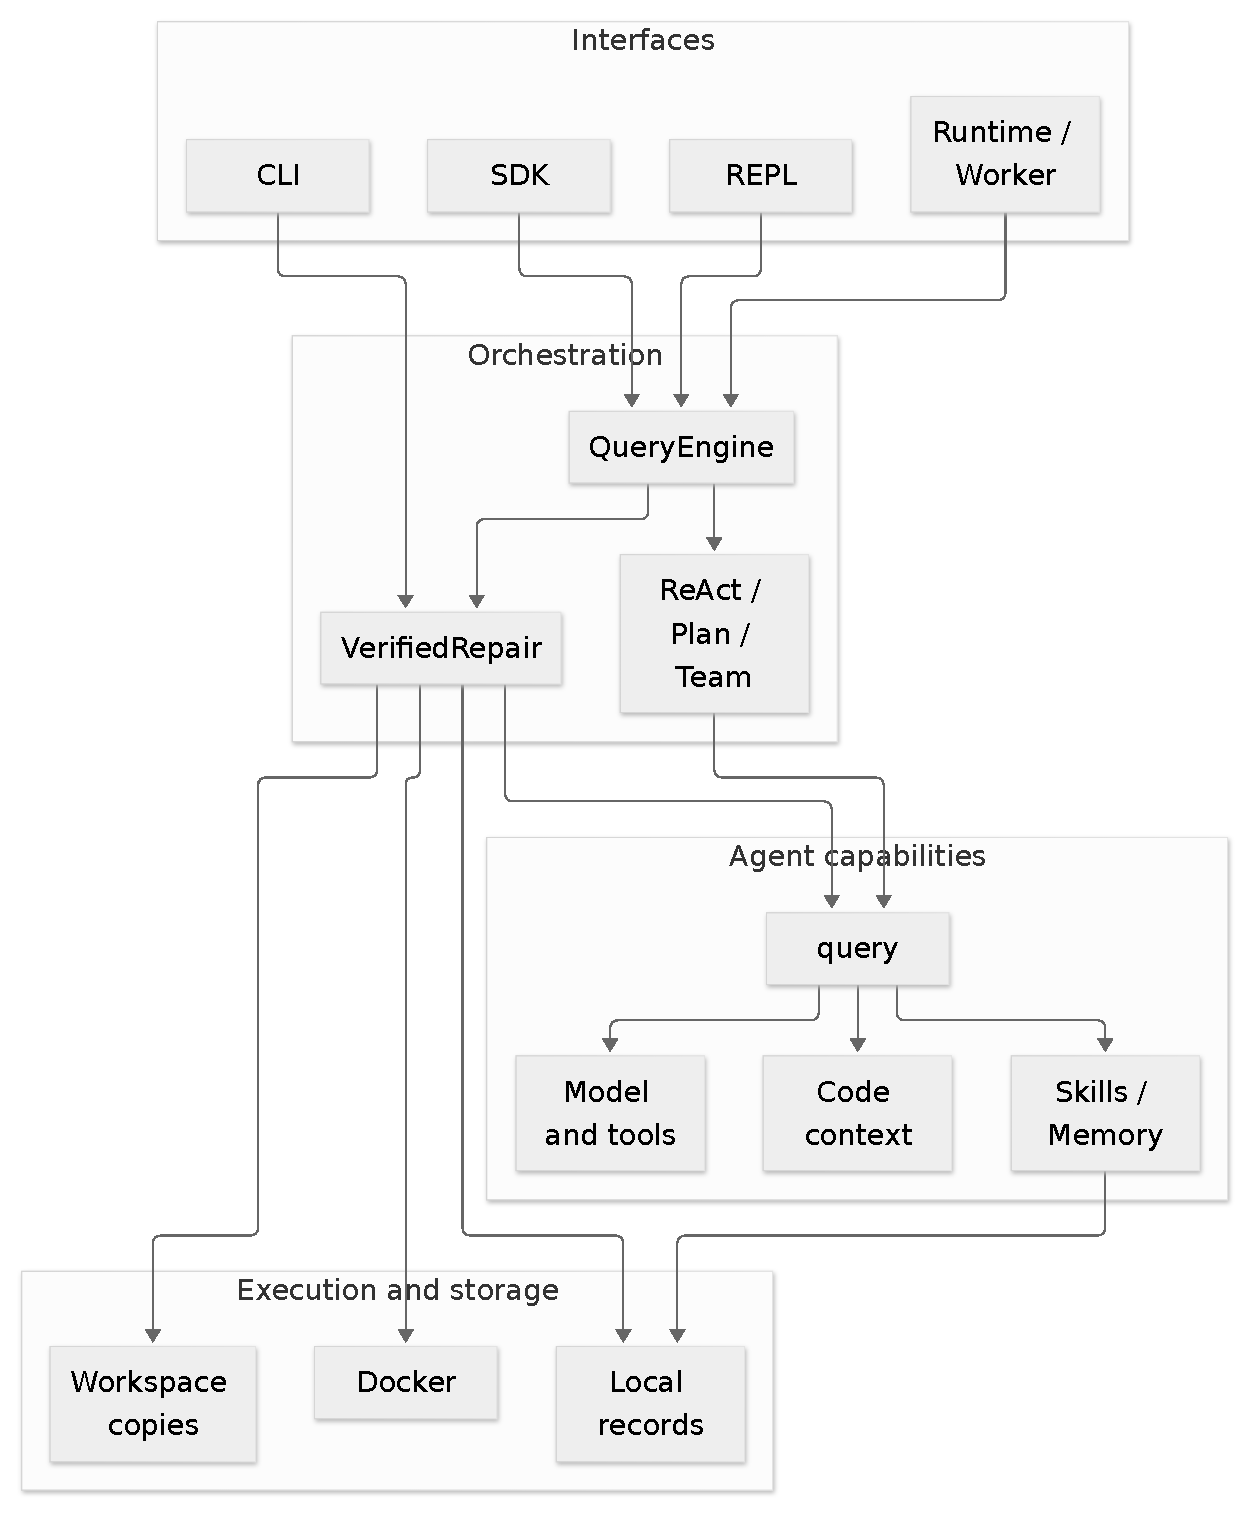
\includegraphics[width=\linewidth,height=0.85\textheight,keepaspectratio]{figures/fig-4-1.pdf}
\caption[System architecture and shared capabilities]{System architecture: general agent modes and dedicated repair share capabilities, while repair owns copies, command constraints and delivery.}\label{fig:4-1}
\end{figure}

General modes retain their original completion rules. A dedicated repair path was chosen to reuse the query loop without treating ordinary model completion as fixed acceptance. Configuration is copied before adjusting tools, paths or policies, leaving the original session unchanged.

Sequential handoffs provide clear candidate ownership through one writer. Concurrent candidates would require independent copies and merge/conflict policies, which were not implemented. CLI constructs \code|VerifiedRepair| directly; the read-evaluate-print loop (REPL), SDK and Runtime use \code|QueryEngine.repair|. These adapters share the repair core without identical invocation paths.

\section{Roles and candidate handoffs}\label{sec:4.2}

Roles are contexts, not necessarily separate models or processes. Table~\ref{tab:4-2} defines their capabilities. Only the worker writes business code; internal read-only indexing may still create technical caches. Arbitrary Model Context Protocol (MCP), web and memory-writing tools are not exposed.

\needspace{14\baselineskip}

\begin{longtable}[]{@{}
  >{\raggedright\arraybackslash}p{(\linewidth - 6\tabcolsep) * \real{0.1400}}
  >{\raggedright\arraybackslash}p{(\linewidth - 6\tabcolsep) * \real{0.3000}}
  >{\raggedright\arraybackslash}p{(\linewidth - 6\tabcolsep) * \real{0.3300}}
  >{\raggedright\arraybackslash}p{(\linewidth - 6\tabcolsep) * \real{0.2300}}@{}}
\caption[Role contracts]{Role capabilities, inputs and handoff artefacts.}\label{tab:4-2}\tabularnewline
\toprule\noalign{}
\begin{minipage}[b]{\linewidth}\raggedright
Role
\end{minipage} & \begin{minipage}[b]{\linewidth}\raggedright
Tools/workspace
\end{minipage} & \begin{minipage}[b]{\linewidth}\raggedright
Input
\end{minipage} & \begin{minipage}[b]{\linewidth}\raggedright
Handoff
\end{minipage} \\
\midrule\noalign{}
\endfirsthead
\toprule\noalign{}
\begin{minipage}[b]{\linewidth}\raggedright
Role
\end{minipage} & \begin{minipage}[b]{\linewidth}\raggedright
Tools/workspace
\end{minipage} & \begin{minipage}[b]{\linewidth}\raggedright
Input
\end{minipage} & \begin{minipage}[b]{\linewidth}\raggedright
Handoff
\end{minipage} \\
\midrule\noalign{}
\endhead
\bottomrule\noalign{}
\endlastfoot
Coordinator & Read/search in work & Task, rules, experience & Concise plan \\
Worker & Read/edit/commands in work & Task, plan, feedback & Actual edits and summary \\
Verifier & Read/search in verify & Task, patch, permitted evidence & Review and suggestions \\
\end{longtable}

Each role receives a fresh history and skill buffer. Retries preserve work files while supplying the latest feedback to a new worker context. Within an attempt, worker completion precedes candidate validation and fixed tests; only then does the verifier receive the reconstructed candidate. Retries repeat the worker-to-verifier stages while budget remains. Actual timestamped instances of these handoffs are examined in Figure~\ref{fig:6-4}, rather than assuming that a design sequence demonstrates executed behaviour.

The verifier interprets evidence but does not supply a machine-authoritative approval. Failing tests cannot be overridden by review. Conversely, passing tests followed by verifier budget exhaustion remain an unsuccessful workflow. Three strategies vary roles and feedback while retaining fixed acceptance; their exact comparison appears in Table~\ref{tab:6-5}.

\section{Files and execution}\label{sec:4.3}

An in-memory initial snapshot records supported paths, bytes and hashes. The worker edits \texttt{work}; each legal candidate reconstructs \texttt{verify}. The source repository is read to establish the baseline, work is the only editable business-code copy, and fixed acceptance receives a read-only verification mount. Reports and patches are exported to a separate delivery directory, not applied automatically to original source. These are distinct ownership boundaries even though all copies originate from the same bytes.

Candidates identify additions, modifications and deletions and reject protected or unsupported content. Verification uses reconstructed bytes, not worker descriptions. Snapshot exclusions and limits protect the supported boundary, not a full operating-system image or universal secret detection.

Each command creates a prepared-image container. Worker commands mount work writable; acceptance mounts verify read-only. Network, capabilities and resources are restricted. Containers do not preserve process state between commands. The host still performs bounded file operations, model communication, indexing and reporting. Unavailable images never trigger host-shell fallback.

\section{States and evidence}\label{sec:4.4}

Reports use JavaScript Object Notation (JSON). They associate source/model/options, baseline, attempts, patches, tests, reviews, skills, memory identifiers and usage. Table~\ref{tab:4-4} lists run states; invalid candidates use attempt-level \code|invalid_patch|.

\begin{longtable}[]{@{}
  >{\raggedright\arraybackslash}p{(\linewidth - 2\tabcolsep) * \real{0.3200}}
  >{\raggedright\arraybackslash}p{(\linewidth - 2\tabcolsep) * \real{0.6800}}@{}}
\caption[Run states]{Run states and their meanings.}\label{tab:4-4}\tabularnewline
\toprule\noalign{}
\begin{minipage}[b]{\linewidth}\raggedright
State
\end{minipage} & \begin{minipage}[b]{\linewidth}\raggedright
Meaning
\end{minipage} \\
\midrule\noalign{}
\endfirsthead
\toprule\noalign{}
\begin{minipage}[b]{\linewidth}\raggedright
State
\end{minipage} & \begin{minipage}[b]{\linewidth}\raggedright
Meaning
\end{minipage} \\
\midrule\noalign{}
\endhead
\bottomrule\noalign{}
\endlastfoot
\texttt{running} & Processing started \\
\code|baseline_passed| & No failing baseline established \\
\texttt{verified} & Acceptance and required handoffs finished \\
\code|environment_error| & Environment failure or command timeout \\
\texttt{no\_progress} & Empty or consecutive repeated candidate \\
\code|attempts_exhausted| & Candidate allowance consumed \\
\code|budget_exhausted| & Model-call or token threshold reached \\
\texttt{timeout} & Overall deadline reached \\
\texttt{canceled} & Repair coroutine cancelled \\
\texttt{error} & Other exception \\
\end{longtable}

\code|report.json| summarises a run, \code|events.jsonl| records ordered activity and \code|attempt-N.patch| preserves legal attempts. Only success exports \code|candidate.patch|. Interrupted attempts may lack later fields. Records support inspection, not full raw-message replay or transactional crash recovery.

\section{Knowledge and interfaces}\label{sec:4.5}

Role-selected reproduction, minimal-change and verification skills are fingerprinted. Memory is recalled once using the original project scope; repair-kind entries must match source. Selected experience is untrusted data, while automatic recall inside temporary copies is disabled. Only successful enabled runs save experience. Warnings do not overwrite test outcomes.

Table~\ref{tab:4-5} summarises interface contracts. Explicit options override configuration; omitted CLI values do not overwrite configured budgets.

\needspace{14\baselineskip}

\begin{longtable}[]{@{}
  >{\raggedright\arraybackslash}p{(\linewidth - 4\tabcolsep) * \real{0.1500}}
  >{\raggedright\arraybackslash}p{(\linewidth - 4\tabcolsep) * \real{0.4300}}
  >{\raggedright\arraybackslash}p{(\linewidth - 4\tabcolsep) * \real{0.4200}}@{}}
\caption[Public entry points]{Entry points and result handling.}\label{tab:4-5}\tabularnewline
\toprule\noalign{}
\begin{minipage}[b]{\linewidth}\raggedright
Interface
\end{minipage} & \begin{minipage}[b]{\linewidth}\raggedright
Invocation
\end{minipage} & \begin{minipage}[b]{\linewidth}\raggedright
Result
\end{minipage} \\
\midrule\noalign{}
\endfirsthead
\toprule\noalign{}
\begin{minipage}[b]{\linewidth}\raggedright
Interface
\end{minipage} & \begin{minipage}[b]{\linewidth}\raggedright
Invocation
\end{minipage} & \begin{minipage}[b]{\linewidth}\raggedright
Result
\end{minipage} \\
\midrule\noalign{}
\endhead
\bottomrule\noalign{}
\endlastfoot
CLI & \code|yecoding repair|, repeatable \code|--test| & Progress/JSON; success exit only if verified \\
REPL & \code|/repair <task>| & Configured tests; separate history \\
SDK & \code|QueryEngine.repair| & Events/report; caller inspects status \\
Runtime & Turn/Task with \code|mode=repair| & Configured tests; unsuccessful report becomes error \\
\end{longtable}

Runtime does not expose every SDK option as a Hypertext Transfer Protocol (HTTP) request field. Queue IDs manage claims, leases and cancellation; repair IDs locate evidence. Cancellation may not immediately interrupt a model request, but late completion cannot overwrite cancelled task state.

% Generated from en/05-core-implementation.md; edit Markdown, then rebuild.
\chapter{Implementation}\label{chap:5}

\section{Shared query loop and restricted tools}\label{sec:5.1}

The asynchronous query generator in \code|agent/query.py| builds instructions, history and tool definitions, then processes text, tool fragments, usage and errors. Calls are reconstructed by index and associated with results by identifier. Tool existence, object inputs and required fields are checked; handlers enforce paths. This is not complete JSON Schema validation.

Adjacent read-only, concurrency-safe calls run under a semaphore; writes preserve ordering. Exceptions become error-marked observations. Repair registries reuse reading, traversal, search and context tools. Only the worker receives editing and command tools. Command schemas remain familiar, but their handlers invoke \code|DockerSandbox.execute| instead of a host shell. The copied configuration restricts MCP and paths without changing the original session.

Python indexing supplies signatures, approximate relationships and selected source. Default context assembly selects up to eight symbols and at most 40 source lines from eligible symbols among the top three. Source spans and truncation distinguish localisation from full implementation coverage; heuristic tokens are separate from provider usage.

Figure~\ref{fig:5-1} tests this packing policy in a fresh, model-free sweep on 26 October 2026: 12 source-labelled understanding tasks on the pinned python-dotenv snapshot, four retrieval strategies and five budgets, producing 240 contexts. The existing evaluation runner supplies every strategy with the same task-author keywords; AST retrieval additionally uses the task query, while the relation ablation retains the same AST query. A symbol is counted as retrieved if its first four source lines intersect a returned span. Body coverage instead measures the fraction of each labelled symbol's full line interval present, averaged within tasks and then across the 12 tasks. These metrics distinguish finding an interface from exposing its implementation.

\begin{figure}[htbp]
\centering
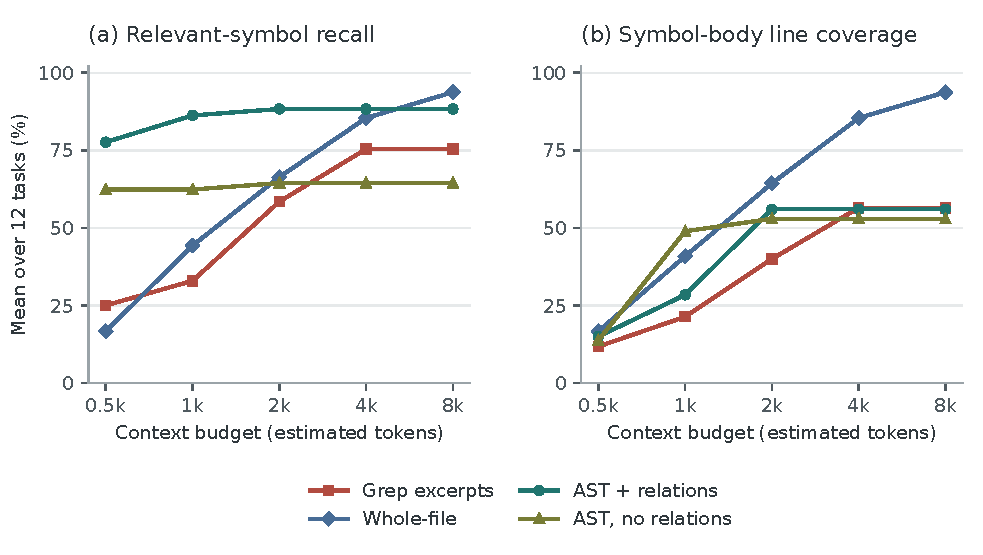
\includegraphics[width=\linewidth,height=0.85\textheight,keepaspectratio]{figures/fig-5-1.pdf}
\caption[Context-budget sensitivity and coverage]{Fresh deterministic retrieval sweep over 12 tasks per point. Left: relevant-symbol recall. Right: coverage of labelled symbol bodies. Budgets use the implemented token estimator, not billed model tokens; no generated-answer or repair-quality scores are measured.}\label{fig:5-1}
\end{figure}

At a 4,000-token allowance, AST with relations retrieves 88.3\% of labelled symbols using a mean 1,243 estimated tokens, compared with 85.4\% and 3,617 for whole-file retrieval: 65.6\% less assembled context, not 65.6\% lower end-to-end model cost. However, AST body coverage is only 56.0\%, versus 85.4\% for whole-file retrieval. Removing relations lowers AST recall to 64.4\%. The 2,000-to-8,000-token plateau exposes the fixed symbol/source-selection caps: extra budget alone cannot recover unselected code. Whole-file recall reaches 93.8\% at 8,000. Thus structural context is useful for compact localisation, but file reads remain necessary for detailed diagnosis; this auxiliary experiment does not establish better repairs.

\section{Source snapshots and candidates}\label{sec:5.2}

\code|RepairWorkspace| records current supported bytes, excluding version control, dependencies, caches and standard private-file patterns. It rejects links, special files and excessive trees. Exact limits are listed in Table~\ref{tab:A-4}. For initial file map \(F_0\), the source fingerprint is:

\begin{equation}
H_0=\operatorname{SHA256}\left(
\mathop{\Vert}_{p\in\operatorname{sort}(\operatorname{keys}(F_0))}
[\operatorname{UTF8}(p)\Vert0x00\Vert\operatorname{SHA256}_{raw}(F_0[p])]
\right).\label{eq:5-1}
\end{equation}

The inner digest contributes raw bytes. SHA-256 is the 256-bit Secure Hash Algorithm; paths use the 8-bit Unicode Transformation Format (UTF-8). Excluded files and environment state are outside this fingerprint. Work persists across attempts; verification is rebuilt from actual candidate bytes, following Algorithm~\ref{alg:5-1}.

\needspace{5\baselineskip}\refstepcounter{thesisalgorithm}\label{alg:5-1}
\noindent\textbf{Algorithm \thethesisalgorithm\quad Candidate validation and verification-copy construction.}\par\nopagebreak

\begin{Verbatim}[fontsize=\normalsize,breaklines=true,breakanywhere=true,frame=single,framesep=2mm]
Input: baseline F0, edited work, verification path
1. Check file types, supported paths and tree limits.
2. F <- bounded snapshot of work.
3. Delta <- sorted content differences between F0 and F.
4. Reject protected changes or non-UTF-8/NUL content.
5. Generate a Git-style unified patch for Delta.
6. Replace verification files with F.
7. Return patch, changed paths and fingerprints.
\end{Verbatim}

Differences use \code|difflib.unified_diff| with creation/deletion and missing-final-newline markers. Content comparison excludes permission-only changes. Host editing rejects protected tests early, while candidate checks catch command-made changes too. Rejection does not restore work automatically: a later attempt must correct it.

Figure~\ref{fig:5-2} gives a concrete candidate from the archived \code|none-value| task. The two added statements preserve existing non-null conversion while correcting null expansion. This connects byte-derived patch delivery to executable evidence rather than a worker summary. The extended suite includes the fixed methods; its 13 passes are not 13 additional independent tests. Chapter~\ref{chap:6} gives the task construction and comparison conditions.

\begin{figure}[htbp]
\centering
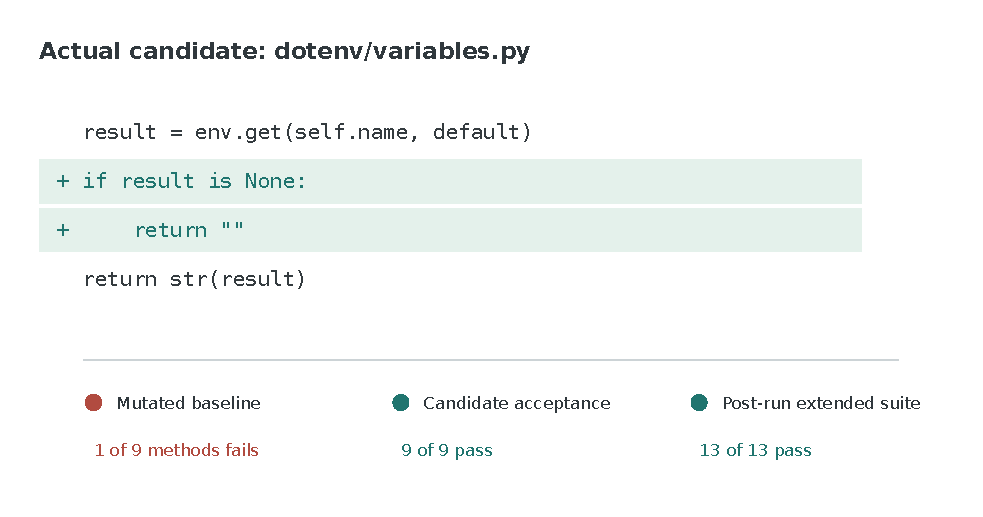
\includegraphics[width=\linewidth,height=0.85\textheight,keepaspectratio]{figures/fig-5-2.pdf}
\caption[Concrete candidate patch and test evidence]{Actual none-value patch excerpt with local indentation and diff addition markers, paired with its archived baseline and candidate checks. Two added statements prevent None becoming text; the post-run 13-method suite includes the nine fixed methods and four additional methods.}\label{fig:5-2}
\end{figure}

\section{Container lifecycle}\label{sec:5.3}

Each command uses a unique container name, a prepared image and argument-list subprocess invocation. Generated text is passed only to the container shell. Network is disabled; root is read-only; capabilities are dropped; limits are one CPU, 512 MiB memory and 128 processes. A roughly 64 MiB temporary filesystem supports writes. Full arguments appear in Table~\ref{tab:A-3}.

Identity follows the host user ID (UID) and group ID (GID), not a universal non-root guarantee. Explicit environment variables disable bytecode writes and third-party pytest plugin autoload. Dependencies must already exist. Worker and acceptance mounts differ in writability.

Output pipes are continuously drained, retaining at most 20,000 bytes per channel. Timeout/cancellation triggers named-container removal and joins output tasks. Cleanup is shielded before cancellation propagates. \code|ExecutionResult.passed| requires exit zero without timeout; diagnostic environment classification is heuristic, and failures never fall back to host execution.

\section{Fixed acceptance and budgets}\label{sec:5.4}

Validation precedes directory creation. A passing baseline ends as \code|baseline_passed|; environment problems remain distinct from test failure. Worker calls allow eight model/tool rounds; other roles allow three. Candidate acceptance is:

\begin{equation}
T_i=\bigwedge_{j=1}^{m}
[(r_{ij}.exit\_code=0)\land\neg r_{ij}.timed\_out].\label{eq:5-2}
\end{equation}

A multi-role workflow additionally requires its verifier call to complete. Algorithm~\ref{alg:5-2} defines the retry sequence.

\needspace{5\baselineskip}\refstepcounter{thesisalgorithm}\label{alg:5-2}
\noindent\textbf{Algorithm \thethesisalgorithm\quad Fixed-acceptance retry under shared budgets.}\par\nopagebreak

\begin{Verbatim}[fontsize=\normalsize,breaklines=true,breakanywhere=true,frame=single,framesep=2mm]
feedback <- baseline; previous_hash <- empty
For each permitted attempt:
  Call worker with task and latest feedback.
  Validate candidate; on rejection, return its reason.
  Stop if changes are empty or repeat previous_hash.
  Save attempt patch; execute all fixed commands.
  Call verifier if required, with permitted evidence.
  If tests passed, export success after handoffs.
  Stop on environment failure or exhausted budget.
  Otherwise return execution/review feedback and retry.
Stop as attempts_exhausted if the loop finishes.
\end{Verbatim}

All roles share one \texttt{BudgetClient}. Product defaults are three attempts, 36 requests, a 60,000-token pre-request threshold, 900 seconds overall and 60 seconds per command. Chapter~\ref{chap:6} reports different experimental request/time limits. The final response can cross the token threshold. Consecutive hashes detect direct repetition, not every longer edit cycle. Unified finalisation records status/usage, removes copies and writes evidence.

\section{Knowledge and delivery}\label{sec:5.5}

Each role owns a skill buffer, with name/version/body hashes recorded. Consumed text can remain in history; one-time injection does not imply no subsequent context cost. The worker cannot dynamically grant itself additional tools through skills.

Memory recall uses original project scope and filters expired entries; repair entries also require a matching \texttt{base\_hash}. Selected text is limited to 6,000 characters. Successful records expire after 30 days and use confidence 0.7 as ranking metadata, not calibrated correctness probability. They state that the patch remains unapplied.

A universally unique identifier (UUID) identifies each delivery. CLI uses only explicit overrides; SDK callers inspect report status; Runtime converts unsuccessful completion to an error and preserves queue cancellation rules. Reports, attempt patches and events retain available evidence, but input rejection or forced termination may prevent complete persistence.

% Generated from en/06-testing-and-evaluation.md; edit Markdown, then rebuild.
\chapter{Testing and Results}\label{chap:6}

\section{Evidence and settings}\label{sec:6.1}

The real-model comparison uses evidence archived on 20 October 2026. Implementation was in an uncommitted workspace based on \texttt{main}, HEAD \code|b90335dbe1e739b2092c846aec59983bfa15ce04|; separate file fingerprints identify evaluated changes. A 26 October supplement reruns model-free retrieval and Docker fixture checks, without changing or repeating the 24 real-model runs. Role-level costs and timelines below are newly reconstructed from their archived event logs. Functional evidence, retrieval behaviour and repair quality have different denominators.

Table~\ref{tab:6-1} fixes the repair conditions. Experimental limits differ from product defaults.

\begin{longtable}[]{@{}
  >{\raggedright\arraybackslash}p{(\linewidth - 2\tabcolsep) * \real{0.2200}}
  >{\raggedright\arraybackslash}p{(\linewidth - 2\tabcolsep) * \real{0.7800}}@{}}
\caption[Experimental configuration]{Configuration shared by the three repair strategies.}\label{tab:6-1}\tabularnewline
\toprule\noalign{}
\begin{minipage}[b]{\linewidth}\raggedright
Item
\end{minipage} & \begin{minipage}[b]{\linewidth}\raggedright
Setting
\end{minipage} \\
\midrule\noalign{}
\endfirsthead
\toprule\noalign{}
\begin{minipage}[b]{\linewidth}\raggedright
Item
\end{minipage} & \begin{minipage}[b]{\linewidth}\raggedright
Setting
\end{minipage} \\
\midrule\noalign{}
\endhead
\bottomrule\noalign{}
\endlastfoot
Source & python-dotenv v1.1.1 production snapshot \\
Source commit & \code|16e660d384b942b11879b44500afbbe021650448| \\
Environment & Prepared \code|python:3.11-slim| image \\
Model & \code|deepseek-v4-flash| \\
Generation & Temperature 0; response allowance capped at 2,048 tokens \\
Acceptance & \code|python -m unittest discover -s tests -v| \\
Run budget & 3 attempts; 18 calls; 60,000-token threshold \\
Deadlines & 180 s body; 60 s per command \\
Knowledge & Skills enabled; cross-task memory disabled \\
Size & 8 held-out defects, 3 strategies, one run/condition: 24 runs \\
\end{longtable}

The archived image is \code|sha256:e88e9763f943ec1834f992a4b51e0f24500486803e8bc534e5767af9ea65f6ce|. Fresh clients and task copies prevent conversational carry-over. The final response can cross the pre-request token threshold. Remote-service variation and concurrent host regression load limit timing interpretation.

\section{Functional verification}\label{sec:6.2}

Table~\ref{tab:6-2} reports archived checks, not newly executed results. The 160 tests comprise 134 existing tests, 25 new repair tests and one snapshot regression.

\begin{longtable}[]{@{}
  >{\raggedright\arraybackslash}p{(\linewidth - 4\tabcolsep) * \real{0.4400}}
  >{\raggedright\arraybackslash}p{(\linewidth - 4\tabcolsep) * \real{0.2800}}
  >{\raggedright\arraybackslash}p{(\linewidth - 4\tabcolsep) * \real{0.2800}}@{}}
\caption[Archived engineering checks]{Archived engineering checks and their scope.}\label{tab:6-2}\tabularnewline
\toprule\noalign{}
\begin{minipage}[b]{\linewidth}\raggedright
Check
\end{minipage} & \begin{minipage}[b]{\linewidth}\raggedright
Result
\end{minipage} & \begin{minipage}[b]{\linewidth}\raggedright
Scope
\end{minipage} \\
\midrule\noalign{}
\endfirsthead
\toprule\noalign{}
\begin{minipage}[b]{\linewidth}\raggedright
Check
\end{minipage} & \begin{minipage}[b]{\linewidth}\raggedright
Result
\end{minipage} & \begin{minipage}[b]{\linewidth}\raggedright
Scope
\end{minipage} \\
\midrule\noalign{}
\endhead
\bottomrule\noalign{}
\endlastfoot
Docker-enabled full pytest run & 160 passed, 28.38 s & Existing and new tests \\
Ruff check & Passed & Static rules \\
Ruff format check & 101 files formatted & Archived state \\
\code|git diff --check| & Passed & Tracked whitespace \\
\code|uv build| & Source/wheel built & Packaging \\
Help, version and doctor & Passed; 0.1.0 & Public CLI \\
\end{longtable}

The full test invocation was \code|YECODING_TEST_DOCKER=1 uv run --extra dev python -m pytest|. Scripted model fixtures produce controlled edits and misleading reviews, while commands execute in real Docker containers. They verify branches without assuming a real model will exhibit a particular failure.

Checks cover source preservation, failed-then-passing retry, protected-test changes through tools and commands, exhausted budgets, missing images, timeout and cancellation cleanup. Sandbox assertions examine environment-variable forwarding, absence of a Docker socket, network and mount restrictions, and bounded output draining. These are functional checks, not a container-escape audit.

A real CLI demonstration on development task \code|default-value| exported a patch and exited successfully. It is excluded from held-out results. SDK/Runtime adaptation checks do not constitute separate real-model comparison suites for every entry point.

\section{Tasks and independent checks}\label{sec:6.3}

Eight production files were taken from pinned python-dotenv source. Each task injects one documented mutation, with an exactly-once original-text match. Table~\ref{tab:6-4} identifies the split. These are synthetic defects, not upstream historical issues or SWE-bench instances.

\begin{longtable}[]{@{}
  >{\raggedright\arraybackslash}p{(\linewidth - 6\tabcolsep) * \real{0.2500}}
  >{\raggedright\arraybackslash}p{(\linewidth - 6\tabcolsep) * \real{0.0900}}
  >{\raggedright\arraybackslash}p{(\linewidth - 6\tabcolsep) * \real{0.1700}}
  >{\raggedright\arraybackslash}p{(\linewidth - 6\tabcolsep) * \real{0.4900}}@{}}
\caption[Injected defects and split]{Development and held-out defects with their mutated behaviours.}\label{tab:6-4}\tabularnewline
\toprule\noalign{}
\begin{minipage}[b]{\linewidth}\raggedright
Task
\end{minipage} & \begin{minipage}[b]{\linewidth}\raggedright
Split
\end{minipage} & \begin{minipage}[b]{\linewidth}\raggedright
File
\end{minipage} & \begin{minipage}[b]{\linewidth}\raggedright
Behaviour
\end{minipage} \\
\midrule\noalign{}
\endfirsthead
\toprule\noalign{}
\begin{minipage}[b]{\linewidth}\raggedright
Task
\end{minipage} & \begin{minipage}[b]{\linewidth}\raggedright
Split
\end{minipage} & \begin{minipage}[b]{\linewidth}\raggedright
File
\end{minipage} & \begin{minipage}[b]{\linewidth}\raggedright
Behaviour
\end{minipage} \\
\midrule\noalign{}
\endhead
\bottomrule\noalign{}
\endlastfoot
\code|default-value| & Dev & \code|variables.py| & Default ignored \\
\code|literal-value| & Dev & \code|variables.py| & Literal lost \\
\code|none-value| & Held-out & \code|variables.py| & Null becomes text \\
\code|trailing-literal| & Held-out & \code|variables.py| & Trailing literal lost \\
\code|variable-cursor| & Held-out & \code|variables.py| & Cursor leaves text \\
\code|unquoted-whitespace| & Held-out & \code|parser.py| & Trailing spaces remain \\
\code|escape-decoding| & Held-out & \code|parser.py| & Escapes not decoded \\
\code|line-tracking| & Held-out & \code|parser.py| & Line number unchanged \\
\code|override-environment| & Held-out & \code|main.py| & Override ignored \\
\code|disable-interpolation| & Held-out & \code|main.py| & Disable switch ignored \\
\end{longtable}

Clean source passed fixed and additional checks. All ten mutated baselines exited 1 as genuine test failures. Fixed acceptance contains nine methods covering the listed behaviours; models may read them but cannot deliver modifications. Four additional methods extend coverage to empty strings, Chinese text, placeholder boundaries, newlines and environment cases.

Post-run assessment applies each available patch in a fresh task copy and installs the additional tests only after model execution. Additional tests and outcomes are never returned to the repairing agents. Both suites were project-authored: independence refers to visibility and execution timing, not independent annotators. On 26 October, a fresh 12-command Docker validation reconfirmed clean fixed/extended-suite passes and genuine failures for all ten mutations using the same prepared image. This refresh establishes fixture validity, not a second sample of model performance.

\section{Strategies and metrics}\label{sec:6.4}

Table~\ref{tab:6-5} defines the conditions within one harness. All retain fixed acceptance. The repair label \texttt{team} is distinct from general Team mode.

\needspace{14\baselineskip}

\begin{longtable}[]{@{}
  >{\raggedright\arraybackslash}p{(\linewidth - 6\tabcolsep) * \real{0.1500}}
  >{\raggedright\arraybackslash}p{(\linewidth - 6\tabcolsep) * \real{0.2000}}
  >{\raggedright\arraybackslash}p{(\linewidth - 6\tabcolsep) * \real{0.3200}}
  >{\raggedright\arraybackslash}p{(\linewidth - 6\tabcolsep) * \real{0.3300}}@{}}
\caption[Comparison strategies]{Roles and candidate feedback in each comparison condition.}\label{tab:6-5}\tabularnewline
\toprule\noalign{}
\begin{minipage}[b]{\linewidth}\raggedright
Strategy
\end{minipage} & \begin{minipage}[b]{\linewidth}\raggedright
Roles
\end{minipage} & \begin{minipage}[b]{\linewidth}\raggedright
Verifier test evidence
\end{minipage} & \begin{minipage}[b]{\linewidth}\raggedright
Later feedback
\end{minipage} \\
\midrule\noalign{}
\endfirsthead
\toprule\noalign{}
\begin{minipage}[b]{\linewidth}\raggedright
Strategy
\end{minipage} & \begin{minipage}[b]{\linewidth}\raggedright
Roles
\end{minipage} & \begin{minipage}[b]{\linewidth}\raggedright
Verifier test evidence
\end{minipage} & \begin{minipage}[b]{\linewidth}\raggedright
Later feedback
\end{minipage} \\
\midrule\noalign{}
\endhead
\bottomrule\noalign{}
\endlastfoot
\texttt{single} & Worker & No verifier & Execution \\
\texttt{team} & Coordinator, worker, verifier & Withheld & Review \\
\texttt{verified} & Coordinator, worker, verifier & Supplied & Execution + review \\
\end{longtable}

For \(N=8\) runs per strategy, terminal state \(s_i\) and additional outcome \(e_i\):

\begin{equation}
R_{workflow}=\frac{1}{N}\sum_{i=1}^{N}\mathbf{1}[s_i=\mathrm{verified}],
\qquad
R_{extra}=\frac{1}{N}\sum_{i=1}^{N}\mathbf{1}[e_i=\mathrm{passed}].\label{eq:6-1}
\end{equation}

Unassessed runs remain in the denominator but are not labelled tested failures. False acceptance means workflow success followed by additional-test failure. Means include failures and cumulative input/output across roles. Duration excludes post-run checks. Strategies ran in manifest order, without randomisation or repetitions; temperature 0 does not establish remote-service determinism.

\section{Outcomes and consumption}\label{sec:6.5}

Table~\ref{tab:6-6} reports workflow completions of eight, five and four. Eighteen runs exported applicable patches; all passed additional checks. Six budget failures exported none and were unassessed. One additional passing patch belonged to an unsuccessful verification-feedback workflow.

Figure~\ref{fig:6-1} retains all 24 task/strategy observations. The three cell categories separate complete workflows, an incomplete workflow with a passing candidate, and runs without an assessable candidate. The last two environment-related tasks exhaust multi-role budgets despite successful single-role completion; the figure also preserves counterexamples instead of reducing each strategy to one percentage.

\begin{figure}[htbp]
\centering
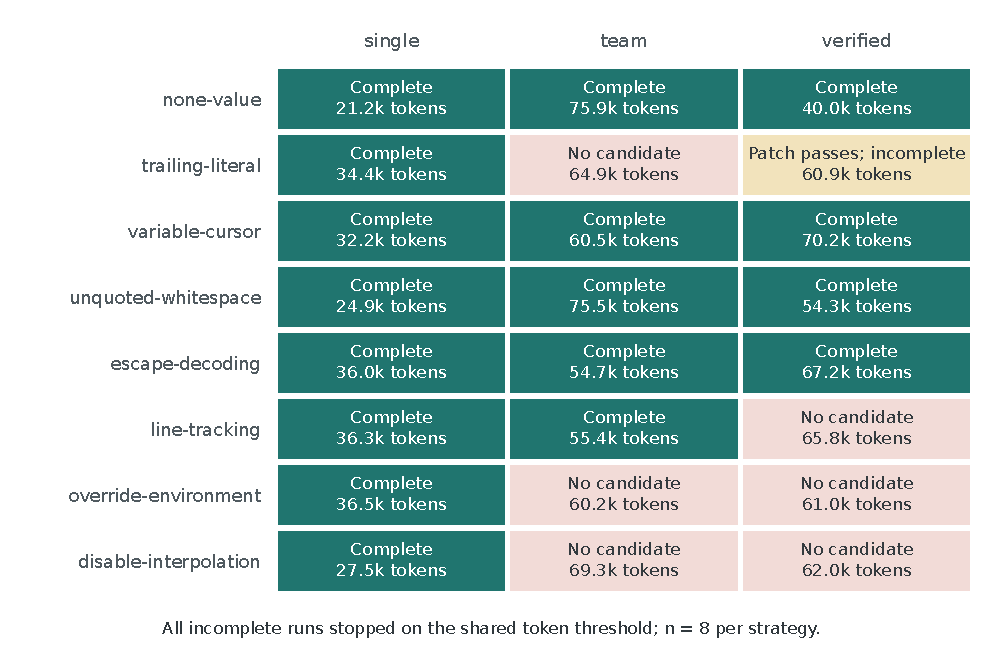
\includegraphics[width=\linewidth,height=0.85\textheight,keepaspectratio]{figures/fig-6-1.pdf}
\caption[Per-task workflow and candidate outcomes]{Outcomes and cumulative tokens for every held-out task/strategy run. Complete means fixed acceptance and required handoffs finished. The amber candidate passed additional checks but its workflow did not finish; no-candidate cells are unassessed, not additional-test failures.}\label{fig:6-1}
\end{figure}

\needspace{14\baselineskip}

\begin{longtable}[]{@{}
  >{\raggedright\arraybackslash}p{(\linewidth - 8\tabcolsep) * \real{0.1600}}
  >{\raggedright\arraybackslash}p{(\linewidth - 8\tabcolsep) * \real{0.2500}}
  >{\raggedright\arraybackslash}p{(\linewidth - 8\tabcolsep) * \real{0.2500}}
  >{\raggedright\arraybackslash}p{(\linewidth - 8\tabcolsep) * \real{0.1800}}
  >{\raggedright\arraybackslash}p{(\linewidth - 8\tabcolsep) * \real{0.1600}}@{}}
\caption[Held-out repair outcomes]{Outcomes across all eight runs per strategy.}\label{tab:6-6}\tabularnewline
\toprule\noalign{}
\begin{minipage}[b]{\linewidth}\raggedright
Strategy
\end{minipage} & \begin{minipage}[b]{\linewidth}\raggedright
Workflow success
\end{minipage} & \begin{minipage}[b]{\linewidth}\raggedright
Extra passes
\end{minipage} & \begin{minipage}[b]{\linewidth}\raggedright
Budget failures
\end{minipage} & \begin{minipage}[b]{\linewidth}\raggedright
False accepts
\end{minipage} \\
\midrule\noalign{}
\endfirsthead
\toprule\noalign{}
\begin{minipage}[b]{\linewidth}\raggedright
Strategy
\end{minipage} & \begin{minipage}[b]{\linewidth}\raggedright
Workflow success
\end{minipage} & \begin{minipage}[b]{\linewidth}\raggedright
Extra passes
\end{minipage} & \begin{minipage}[b]{\linewidth}\raggedright
Budget failures
\end{minipage} & \begin{minipage}[b]{\linewidth}\raggedright
False accepts
\end{minipage} \\
\midrule\noalign{}
\endhead
\bottomrule\noalign{}
\endlastfoot
\texttt{single} & 8/8 (100.0\%) & 8/8 (100.0\%) & 0/8 & 0 \\
\texttt{team} & 5/8 (62.5\%) & 5/8 (62.5\%) & 3/8 & 0 \\
\texttt{verified} & 4/8 (50.0\%) & 5/8 (62.5\%) & 4/8 & 0 \\
\end{longtable}

No candidate passed fixed tests and failed additional checks. Therefore, zero observed false acceptance does not isolate a verifier benefit or establish zero risk. All strategies shared the same acceptance gate.

Table~\ref{tab:6-7} reports aggregate consumption; Figure~\ref{fig:6-2} pairs the three observations for each task to retain within-task differences. Mean multi-role tokens were approximately 2.07 and 1.93 times the single-role value. Values above 60,000 reflect pre-request checking, not a violated hard response cap. A completed final response can cross the threshold without another request being made.

\needspace{14\baselineskip}

\begin{longtable}[]{@{}
  >{\raggedright\arraybackslash}p{(\linewidth - 6\tabcolsep) * \real{0.1700}}
  >{\raggedright\arraybackslash}p{(\linewidth - 6\tabcolsep) * \real{0.2600}}
  >{\raggedright\arraybackslash}p{(\linewidth - 6\tabcolsep) * \real{0.3000}}
  >{\raggedright\arraybackslash}p{(\linewidth - 6\tabcolsep) * \real{0.2700}}@{}}
\caption[Mean resource consumption]{Mean consumption over all runs, with token totals rounded to integers.}\label{tab:6-7}\tabularnewline
\toprule\noalign{}
\begin{minipage}[b]{\linewidth}\raggedright
Strategy
\end{minipage} & \begin{minipage}[b]{\linewidth}\raggedright
Tokens
\end{minipage} & \begin{minipage}[b]{\linewidth}\raggedright
Calls
\end{minipage} & \begin{minipage}[b]{\linewidth}\raggedright
Body duration (s)
\end{minipage} \\
\midrule\noalign{}
\endfirsthead
\toprule\noalign{}
\begin{minipage}[b]{\linewidth}\raggedright
Strategy
\end{minipage} & \begin{minipage}[b]{\linewidth}\raggedright
Tokens
\end{minipage} & \begin{minipage}[b]{\linewidth}\raggedright
Calls
\end{minipage} & \begin{minipage}[b]{\linewidth}\raggedright
Body duration (s)
\end{minipage} \\
\midrule\noalign{}
\endhead
\bottomrule\noalign{}
\endlastfoot
\texttt{single} & 31,120 & 5.750 & 13.44 \\
\texttt{team} & 64,541 & 9.125 & 17.00 \\
\texttt{verified} & 60,167 & 9.750 & 18.06 \\
\end{longtable}

\begin{figure}[htbp]
\centering
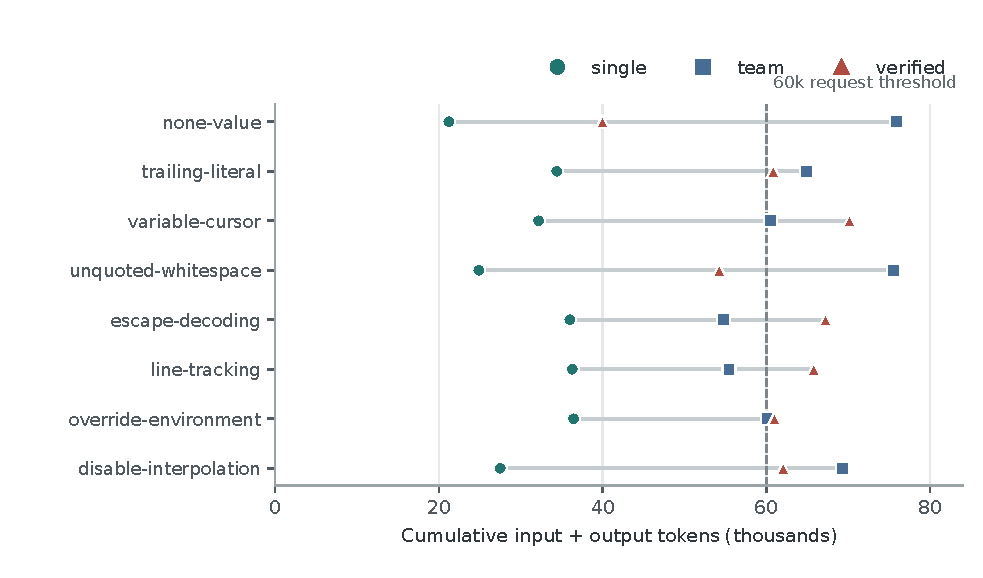
\includegraphics[width=\linewidth,height=0.85\textheight,keepaspectratio]{figures/fig-6-2.pdf}
\caption[Paired per-task model-token costs]{Paired cumulative model-token consumption on the same eight tasks, including failures. Each row joins observations for one task, not repeated samples. The dashed line is a pre-request stopping threshold, not a hard cap on the final response.}\label{fig:6-2}
\end{figure}

Figure~\ref{fig:6-3} attributes every recorded usage event to its active role. Summed role tokens exactly reconcile with report totals for all 24 runs. Averaging all eight runs per strategy, coordinator/worker/verifier consumption is 19.4k/28.2k/16.9k for review feedback and 20.4k/31.4k/8.3k for verification feedback. Non-worker roles account for 56.3\% and 47.7\% of total consumption respectively. Single-role worker consumption is 31.1k, close to the verification-feedback worker's 31.4k; the additional roles therefore identify a concrete resource burden rather than an unexplained aggregate increase.

\begin{figure}[htbp]
\centering
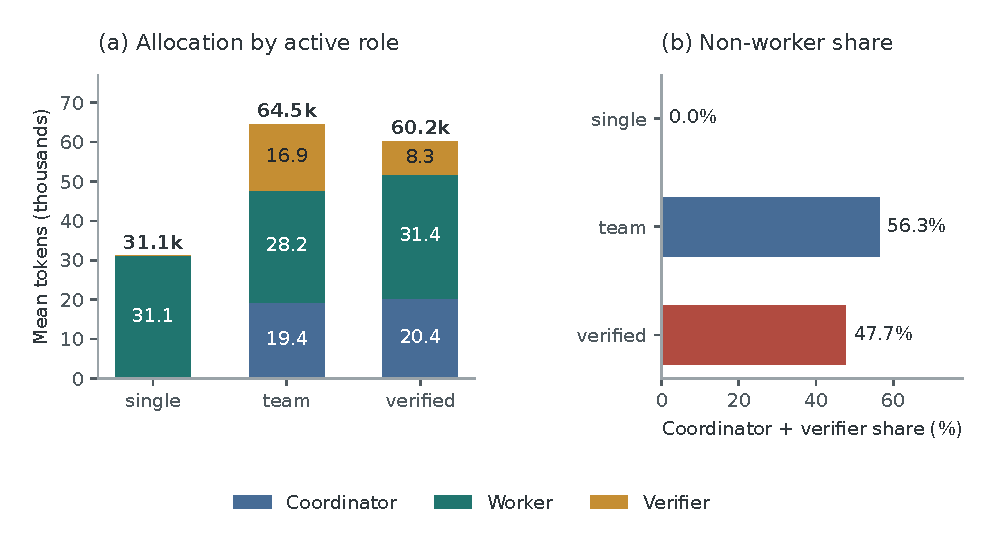
\includegraphics[width=\linewidth,height=0.85\textheight,keepaspectratio]{figures/fig-6-3.pdf}
\caption[Model-token allocation by role]{Mean cumulative tokens attributed to active roles, including failures, and the proportion consumed outside the worker. Input tokens include repeated prompts and tool history; values are usage accounting, not unique source tokens or an isolated causal estimate of role overhead.}\label{fig:6-3}
\end{figure}

Lower verifier usage is not necessarily efficiency: six multi-role runs stop before candidate handoff and never reach that role. These observed allocations motivate budget reservation or selective review as future experiments; they do not demonstrate that either modification would improve completion.

Timing includes model response, container startup, host load and early stopping. Faster failure is not faster completion of equivalent work. No stable latency ratio or production throughput is inferred.

\section{Cases and failure stages}\label{sec:6.6}

For \code|none-value|, the single-role worker added a null check before \code|str(result)| in \code|dotenv/variables.py|, as shown in Figure~\ref{fig:5-2}. One file changed; all nine fixed and 13 extended methods passed, using five calls and 21,220 tokens. The candidate was behaviourally valid under these checks without reproducing the upstream statement verbatim.

For \code|trailing-literal|, verification feedback restored \code|if cursor < length| and passed fixed tests. The verifier then reached the token threshold: 11 calls and 60,863 tokens. \code|attempt-1.patch| remained available and passed post-run checks, but no successful \code|candidate.patch| was delivered. Retrospectively changing this failure to success would alter the predefined completion policy.

Figure~\ref{fig:6-4} reconstructs two verification-feedback runs from elapsed event times. Shading denotes actual role intervals, while the staircase accumulates provider-reported usage when events arrive. The test marker is verifier entry immediately after successful fixed tests, not an exact test-completion timestamp. In \code|trailing-literal|, the worker finishes at 14.50 s and review starts at 16.37 s; the candidate is already test-passing, but review cannot finish within budget. This localises a failure that the success percentage alone cannot explain. The comparison is diagnostic, not a controlled latency benchmark.

\begin{figure}[htbp]
\centering
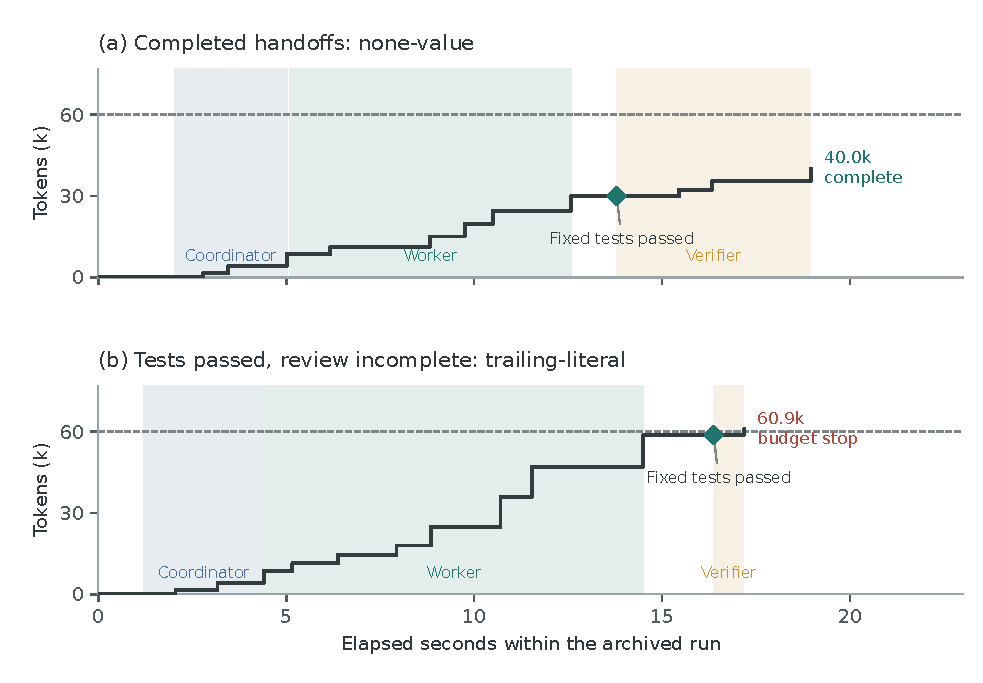
\includegraphics[width=\linewidth,height=0.85\textheight,keepaspectratio]{figures/fig-6-4.pdf}
\caption[Actual execution and budget trajectories]{Event-derived cumulative-token traces for a completed and an incomplete verification-feedback run. Role bands use logged entry/exit times; the unfinished review band ends at run termination. The test diamond marks the post-test verifier entry, and the horizontal line is the 60k request threshold.}\label{fig:6-4}
\end{figure}

The other six failures started the worker but never returned to candidate export. They are not six independently disproved patches. All seven failures exhausted tokens before the 18-call limit. Every run created one attempt only, so real-model results do not establish a multi-round feedback gain. Table~\ref{tab:A-1} preserves task-level outcomes; Chapter~\ref{chap:7} interprets their limits.

% Generated from en/07-discussion.md; edit Markdown, then rebuild.
\chapter{Discussion}\label{chap:7}

This chapter interprets the observations in Chapter~\ref{chap:6} against the specification and research questions. It separates engineering capability from repair-quality evidence and identifies the limits of the comparison.

\section{Assessment against the specification}\label{sec:7.1}

The archived checks support a working integration of the original coding loop with dedicated repair boundaries. Role-specific registries preserve reading, searching and editing while constraining writable files and command execution. Source snapshots and disposable copies associate patches with an input state and avoid automatic changes to the original repository. Timeout and cancellation tests support the implemented cleanup paths.

These observations address RQ1 within the supported Python setting. The boundary is layered: host file checks, candidate validation and container restrictions each perform a different function. A container cannot replace host path checks. Nor does repair-path testing establish equivalent isolation for general ReAct, Plan or Team modes. The evidence is functional validation of specified controls rather than proof against arbitrary malicious code.

For RQ2, actual candidate files, fixed command results and reviews are associated within the same run. Tests remain authoritative even if a model claims success. Passing baselines, invalid candidates, no progress and unavailable environments are not relabelled as repaired defects. These behaviours meet the central requirement to distinguish model statements from execution evidence.

The retry mechanism also has functional evidence: controlled fixtures exercise a failed candidate followed by a successful one. However, no real-model held-out run entered a second attempt. Functional support for retry must therefore not be described as observed quality improvement through repeated model feedback.

\section{Candidate behaviour and workflow completion}\label{sec:7.2}

The \code|trailing-literal| case demonstrates why patch behaviour and workflow completion require separate records. The candidate passed fixed and additional tests, but the verifier could not finish within the shared token threshold. It was correctly reported as an unsuccessful workflow under the implemented completion rule.

Requiring all handoffs to finish makes process completeness explicit, yet adds cost after a candidate already passes acceptance. A future strategy could choose review by risk or reserve verifier budget, but such a change would alter the policy and must be evaluated separately. The current data do not establish that either optimisation would be effective.

Likewise, absence of a patch means additional checks were unavailable, not that a candidate failed them. Preserving this distinction avoids assigning behavioural failure to incomplete interaction. Evidence fields and termination states should be interpreted together rather than collapsed into one success flag.

\section{Collaboration and resource trade-offs}\label{sec:7.3}

The single-role strategy completed all eight held-out tasks; multi-role review and verification feedback completed five and four. The latter used approximately 2.07 and 1.93 times the single-role mean tokens. Under these conditions, extra coordination and inspection did not produce a completion advantage.

The event-derived allocation sharpens this observation: coordinator and verifier contexts consume 56.3\% of review-feedback tokens and 47.7\% of verification-feedback tokens. Worker consumption alone is not substantially lower in the verification-feedback condition. However, these are observed accounting shares, not a counterfactual estimate: some workers stop early, repeated input contributes to every role, and the tasks were not repeated. The failed post-test review in Figure~\ref{fig:6-4} identifies one policy-sensitive stopping point, not proof that removing review is generally preferable.

The defects usually required local condition or assignment changes, with clear behavioural descriptions. Planning and repeated inspection could consume a substantial share of the allowance without requiring a cross-file design decision. This is consistent with the recorded budget failures, but is an interpretation rather than an isolated causal effect.

All strategies retained fixed acceptance, and none exhibited a fixed-test pass followed by an extra-test failure. Consequently, observed zero false acceptance cannot be credited specifically to the verifier or used to rank strategies on detecting inadequately tested patches. More challenging independent tasks would be needed to expose such differences.

The shared budget measures the overall trade-off of the current workflows, not performance after arbitrary retuning. Giving more calls or tokens to one strategy after seeing failures would define a new experiment. The original outcomes and all-run resource means have therefore been retained.

The observations should also be placed against the repair literature. GenProg and Nopol differ substantially from LLM-based editing, yet retain the separation between candidate construction and executable constraints. Their results do not predict the ranking of the present strategies. Patch-assessment studies explain why passing the guiding suite remains a limited claim; the present extra tests provide only a small additional behavioural sample, not those studies' complete assessment methods. The useful comparison is therefore methodological: which evidence is retained and what it can establish, rather than whose published success percentage is larger. \citep{legoues2012genprog, xuan2017nopol, ye2021assessment}

\section{Threats to validity}\label{sec:7.4}

\subsection{Tasks and coverage}\label{sec:7.4.1}

Only eight held-out mutations were evaluated, from one repository and three production files. They do not cover complex concurrency, dependency preparation, long diagnosis or broad cross-file changes. The observed 8/8 single-role completion is not an estimate for arbitrary repair tasks and does not imply that multi-agent collaboration is generally ineffective.

Development and held-out splits prevent development cases from being included directly in the reported denominator. However, the same project produced tasks and tests, without independent expert validation. The shared fixed suite also covers development-task behaviours. This is held-out defect evaluation under shared acceptance, not comprehensive generalisation to unseen repositories and test distributions.

Additional tests cover finite behaviours and may miss defects. Their independence is operational visibility and timing, not independent authorship. Passing them does not prove full upstream semantics.

Pinned source improves repeatability but does not establish that the model has never encountered the library or related repair patterns during training. Clear task descriptions may also expose substantial localisation information. No training-data contamination measurement was performed, so apparent repair competence cannot be separated from prior familiarity in this corpus. Broader, independently constructed tasks would be needed to examine that distinction. This is another reason to avoid equating a benchmark identity, a repository snapshot and an unseen reasoning challenge. \citep{legoues2015manybugs, wong2016localization}

\subsection{Experimental design}\label{sec:7.4.2}

There was one run per task/strategy, no randomisation of condition order and incomplete control over remote-model changes or host load. Repeated-run variance and statistical significance cannot be inferred. Temperature 0 does not eliminate service variation.

Common budgets impose different practical constraints on workflows needing different numbers of calls. Results describe that chosen operating point, not every possible budget allocation. No real-model second attempt occurred, limiting conclusions about the difference between review and verification feedback on retries. Duration is descriptive and does not support strict performance ratios.

\subsection{Knowledge and traceability}\label{sec:7.4.3}

Skills were enabled and cross-task memory disabled throughout the real-model experiment. Functional tests support loading, provenance, filtering and saving, but no independent knowledge-feature ablation establishes improved repair rates. Earlier AST context experiments likewise do not establish end-to-end repair gains here.

The fresh budget sweep in Figure~\ref{fig:5-1} measures a narrower property: localisation and line exposure under a deterministic context packer. Its plateau and whole-file crossover show why compact symbol recall cannot substitute for inspecting implementation. The task labels and fixed query terms remain project-authored, the corpus is small and no new model-generated answer is scored. These findings support a design trade-off, not an end-to-end repair improvement or reduced billed-token claim.

Fingerprints cover supported source files, not the full image, dependencies or remote service. Reports omit some raw model interactions and hardware state. They support delivery inspection and process analysis without guaranteeing exact model-output reproduction or recovery after arbitrary process failure.

\section{Implications}\label{sec:7.5}

The strongest supported contribution is an executable repair architecture with explicit evidence, boundaries and failure reporting. More roles should be justified by observed task benefit relative to their total cost. Candidate checks, acceptance evidence and stopping policies must be assessed together. A negative completion result remains useful because it identifies where the current orchestration spends resources and what a subsequent experiment must test.

% Generated from en/08-conclusion-and-future-work.md; edit Markdown, then rebuild.
\chapter{Conclusions and Further Work}\label{chap:8}

\section{Achievements}\label{sec:8.1}

This dissertation designed and implemented a dedicated collaboration and verification workflow on an existing Python terminal coding agent. It reused the model protocol, tool loop, repository retrieval and knowledge facilities, while adding role-specific execution boundaries, disposable copies, candidate validation, fixed acceptance and evidence delivery.

Coordinator, worker and verifier contexts interact sequentially, with a single writer. Host file checks, source snapshots and restricted Docker commands protect the supported task boundary. Patches are exported rather than applied automatically. Tests, reviews, usage and termination causes are associated with actual candidates. Shared attempts, calls, token thresholds and time limits control retries and unsuccessful execution.

Procedural skills guide reproduction, minimal changes and verification. Project memory stores attributable experience with source fingerprints and expiry. These inputs cannot override current acceptance. CLI, REPL, SDK and Runtime adapters expose the same core while retaining their different result and cancellation contracts.

Archived verification reports 160 passing automated tests, including existing regressions. The controlled experiment used ten injected defects in pinned python-dotenv source, with two development and eight held-out tasks and 24 real-model runs. Post-run checks inspected available patches without feeding their results back to the agents.

\section{Conclusions against the research questions}\label{sec:8.2}

For RQ1, restricted role registries, disposable copies and containers demonstrate a practical way to retain coding capabilities while bounding supported repair changes. The original source is not automatically modified, and functional checks cover cleanup and access constraints. This conclusion concerns the implemented mechanisms, not universal security.

For RQ2, fixed executor results provide acceptance independently of model claims. Candidate patches, reviews and termination records make incomplete outcomes inspectable. The observed passing candidate in a budget-failed workflow confirms that candidate behaviour and process completion must be reported separately. Bounded retry is functionally implemented, but a real-model multi-round improvement remains untested.

For RQ3, single-role, review-feedback multi-role and verification-feedback multi-role strategies completed eight, five and four tasks respectively. Additional checks passed for eight, five and five runs; all seven failures exhausted token budgets. The current experiment does not show a multi-role success-rate advantage. It instead records the coordination cost of the implemented strategies on small local defects.

The work therefore establishes a functioning and inspectable repair workflow and a bounded empirical assessment of its trade-offs. Engineering completeness does not imply superior repair quality, and the limited negative result does not establish that multiple agents are universally ineffective.

\section{Further work}\label{sec:8.3}

\subsection{Independent tasks and repeated evaluation}\label{sec:8.3.1}

A subsequent dataset should include more repositories, cross-file dependencies and real historical defects, with independently reviewed tasks and acceptance conditions. Budgets and success definitions should be frozen before repeated runs, with randomised condition order and consistent all-run denominators.

Tasks in which a plausible first candidate genuinely fails would test whether subsequent evidence improves repair. Scripted functional tests should continue to cover branches reliably, while real-model experiments separately assess actual outcomes.

\subsection{Role selection and budget allocation}\label{sec:8.3.2}

Risk-based role selection, reserved stage budgets, compact handoffs and on-demand retrieval could reduce repeated input or avoid exhausting resources before final inspection. These are hypotheses requiring new controlled comparisons of completion, false acceptance and consumption.

Changing whether review remains mandatory after passing tests also changes completion policy and must be reported as a separate condition. Parallel candidate generation would require independent copies, candidate ownership and conflict handling, rather than multiple writers in a shared directory.

\subsection{Skills and memory}\label{sec:8.3.3}

Separate skills-on/off and memory-on/off comparisons are needed to assess quality and cost. Project/time splits should prevent previous answers leaking into evaluation. Irrelevant retrieval, incorrect experience and stale-entry filtering should be measured alongside successful reuse. Environment and dependency fingerprints could extend applicability checks, but current integration does not guarantee a benefit.

\subsection{Delivery and inspection}\label{sec:8.3.4}

Additional environment metadata, request summaries and per-stage usage could improve diagnosis under explicit retention and credential-handling rules. Interrupted report writes, patch replay and source checks before manual application also merit stronger delivery protocols. The objective is sufficient evidence for inspection rather than unlimited retention of source and private data.

\section{Closing conclusion}\label{sec:8.4}

Reliable assessment requires a clear relationship between source changes, executable evidence, resource expenditure and termination. The implemented workflow provides that relationship within its supported scope. Further improvements should be judged by measurable task outcomes rather than role count alone.

\clearpage
\phantomsection
\addcontentsline{toc}{chapter}{References}
\renewcommand{\bibname}{References}
\setlength{\bibsep}{0pt}
\bibliographystyle{unsrtnat}
\bibliography{references}
\clearpage
\appendix
% Generated from en/appendix-artefacts.md; edit Markdown, then rebuild.
\chapter{Supporting Details and Project Records}\label{app:artefacts}

\section{Per-task results}\label{per-task-results}

Table~\ref{tab:A-1} supplements the aggregate results in Chapter~\ref{chap:6}. Each cell pairs the recorded workflow status with the post-run check outcome. Budget means token-budget termination; not checked means no exported patch.

\begin{longtable}[]{@{}
  >{\raggedright\arraybackslash}p{(\linewidth - 6\tabcolsep) * \real{0.3700}}
  >{\raggedright\arraybackslash}p{(\linewidth - 6\tabcolsep) * \real{0.2100}}
  >{\raggedright\arraybackslash}p{(\linewidth - 6\tabcolsep) * \real{0.2100}}
  >{\raggedright\arraybackslash}p{(\linewidth - 6\tabcolsep) * \real{0.2100}}@{}}
\caption[Per-task outcomes]{Workflow and additional-test outcomes for the eight held-out injected defects.}\label{tab:A-1}\tabularnewline
\toprule\noalign{}
\begin{minipage}[b]{\linewidth}\raggedright
Task
\end{minipage} & \begin{minipage}[b]{\linewidth}\raggedright
\texttt{single}
\end{minipage} & \begin{minipage}[b]{\linewidth}\raggedright
\texttt{team}
\end{minipage} & \begin{minipage}[b]{\linewidth}\raggedright
\texttt{verified}
\end{minipage} \\
\midrule\noalign{}
\endfirsthead
\toprule\noalign{}
\begin{minipage}[b]{\linewidth}\raggedright
Task
\end{minipage} & \begin{minipage}[b]{\linewidth}\raggedright
\texttt{single}
\end{minipage} & \begin{minipage}[b]{\linewidth}\raggedright
\texttt{team}
\end{minipage} & \begin{minipage}[b]{\linewidth}\raggedright
\texttt{verified}
\end{minipage} \\
\midrule\noalign{}
\endhead
\bottomrule\noalign{}
\endlastfoot
\code|none-value| & Success/pass & Success/pass & Success/pass \\
\code|trailing-literal| & Success/pass & Budget/not checked & Budget/pass \\
\code|variable-cursor| & Success/pass & Success/pass & Success/pass \\
\code|unquoted-whitespace| & Success/pass & Success/pass & Success/pass \\
\code|escape-decoding| & Success/pass & Success/pass & Success/pass \\
\code|line-tracking| & Success/pass & Success/pass & Budget/not checked \\
\code|override-environment| & Success/pass & Budget/not checked & Budget/not checked \\
\code|disable-interpolation| & Success/pass & Budget/not checked & Budget/not checked \\
\end{longtable}

\section{Functional traceability}\label{functional-traceability}

Table~\ref{tab:A-2} expands the essential acceptance conditions specified in Chapter~\ref{chap:3}. Functional checks do not establish an independent repair-quality gain.

\begin{longtable}[]{@{}
  >{\raggedright\arraybackslash}p{(\linewidth - 6\tabcolsep) * \real{0.1000}}
  >{\raggedright\arraybackslash}p{(\linewidth - 6\tabcolsep) * \real{0.2500}}
  >{\raggedright\arraybackslash}p{(\linewidth - 6\tabcolsep) * \real{0.4300}}
  >{\raggedright\arraybackslash}p{(\linewidth - 6\tabcolsep) * \real{0.2200}}@{}}
\caption[Acceptance traceability]{Functional acceptance scenarios and their requirement mappings.}\label{tab:A-2}\tabularnewline
\toprule\noalign{}
\begin{minipage}[b]{\linewidth}\raggedright
ID
\end{minipage} & \begin{minipage}[b]{\linewidth}\raggedright
Scenario
\end{minipage} & \begin{minipage}[b]{\linewidth}\raggedright
Expected condition
\end{minipage} & \begin{minipage}[b]{\linewidth}\raggedright
Requirements
\end{minipage} \\
\midrule\noalign{}
\endfirsthead
\toprule\noalign{}
\begin{minipage}[b]{\linewidth}\raggedright
ID
\end{minipage} & \begin{minipage}[b]{\linewidth}\raggedright
Scenario
\end{minipage} & \begin{minipage}[b]{\linewidth}\raggedright
Expected condition
\end{minipage} & \begin{minipage}[b]{\linewidth}\raggedright
Requirements
\end{minipage} \\
\midrule\noalign{}
\endhead
\bottomrule\noalign{}
\endlastfoot
AC-01 & Missing commands & Reject before model repair & FR-03, FR-04 \\
AC-02 & Passing baseline & No new-repair claim & FR-04, FR-06 \\
AC-03 & Failed then valid candidate & Feedback, patch/report, source unchanged & FR-05 to FR-08 \\
AC-04 & Positive review, failing tests & Preserve failure and bounded retry & FR-06, FR-07 \\
AC-05 & Protected or out-of-scope edit & Reject operation or candidate & FR-01, FR-06 \\
AC-06 & Budget/no progress & Explicit stop and available evidence & FR-07, FR-08 \\
AC-07 & Timeout, cancellation, missing image & Cleanup; no host fallback & NFR-02, NFR-04 \\
AC-08 & Skills/memory & Attributable input; filtering; disabled mode & FR-09, FR-10 \\
AC-09 & Entry change/late result & Shared acceptance; cancelled state retained & FR-03, NFR-05 \\
\end{longtable}

\section{Execution parameters}\label{execution-parameters}

Table~\ref{tab:A-3} lists container arguments supporting the boundary described in Chapters4 and5. These are implemented settings, not proof of universal isolation.

\begin{longtable}[]{@{}
  >{\raggedright\arraybackslash}p{(\linewidth - 4\tabcolsep) * \real{0.2200}}
  >{\raggedright\arraybackslash}p{(\linewidth - 4\tabcolsep) * \real{0.4700}}
  >{\raggedright\arraybackslash}p{(\linewidth - 4\tabcolsep) * \real{0.3100}}@{}}
\caption[Container arguments]{Container arguments and their intended execution constraints.}\label{tab:A-3}\tabularnewline
\toprule\noalign{}
\begin{minipage}[b]{\linewidth}\raggedright
Mechanism
\end{minipage} & \begin{minipage}[b]{\linewidth}\raggedright
Setting
\end{minipage} & \begin{minipage}[b]{\linewidth}\raggedright
Effect
\end{minipage} \\
\midrule\noalign{}
\endfirsthead
\toprule\noalign{}
\begin{minipage}[b]{\linewidth}\raggedright
Mechanism
\end{minipage} & \begin{minipage}[b]{\linewidth}\raggedright
Setting
\end{minipage} & \begin{minipage}[b]{\linewidth}\raggedright
Effect
\end{minipage} \\
\midrule\noalign{}
\endhead
\bottomrule\noalign{}
\endlastfoot
Image/lifecycle & \code|--pull=never|, \code|--rm|, unique name & Prepared image; cleanup \\
Network/root & \code|--network=none|, \code|--read-only| & No network; restricted writes \\
Privileges & \code|--cap-drop=ALL|, \code|no-new-privileges| & Reduced authority \\
Resources & \code|--cpus=1|, \code|--memory=512m|, \code|--pids-limit=128| & Per-command bounds \\
Identity & Host UID and GID & Deployment-dependent identity \\
Temporary files & Approximately 64 MiB tmpfs at \code|/tmp| & Bounded writes \\
Workspace & Selected copy at \code|/workspace| & Task source mount \\
Environment/logs & Explicit variables; Docker logging disabled & Limited forwarding/storage \\
\end{longtable}

Table~\ref{tab:A-4} specifies bounded source handling. The source fingerprint covers supported files only.

\begin{longtable}[]{@{}
  >{\raggedright\arraybackslash}p{(\linewidth - 4\tabcolsep) * \real{0.2300}}
  >{\raggedright\arraybackslash}p{(\linewidth - 4\tabcolsep) * \real{0.4300}}
  >{\raggedright\arraybackslash}p{(\linewidth - 4\tabcolsep) * \real{0.3400}}@{}}
\caption[Snapshot limits]{Snapshot and candidate limits used by the repair workspace.}\label{tab:A-4}\tabularnewline
\toprule\noalign{}
\begin{minipage}[b]{\linewidth}\raggedright
Check
\end{minipage} & \begin{minipage}[b]{\linewidth}\raggedright
Limit or rule
\end{minipage} & \begin{minipage}[b]{\linewidth}\raggedright
Purpose
\end{minipage} \\
\midrule\noalign{}
\endfirsthead
\toprule\noalign{}
\begin{minipage}[b]{\linewidth}\raggedright
Check
\end{minipage} & \begin{minipage}[b]{\linewidth}\raggedright
Limit or rule
\end{minipage} & \begin{minipage}[b]{\linewidth}\raggedright
Purpose
\end{minipage} \\
\midrule\noalign{}
\endhead
\bottomrule\noalign{}
\endlastfoot
Individual file & 2,000,000 bytes & Bound reads \\
Total bytes & 100,000,000 & Bound memory \\
Snapshot files & 10,000 & Bound scope \\
Safety traversal & 20,000 entries & Bound generated tree \\
Types/names & No links, special files or unsupported path characters & Avoid traversal/diff ambiguity \\
Protected files & Tests and selected configuration & Preserve acceptance \\
\end{longtable}

\section{Artefact locations}\label{artefact-locations}

\begin{itemize}
\tightlist
\item
  Repair orchestration: \code|src/yecoding/agent/repair.py|.
\item
  Workspace and command execution: \code|src/yecoding/sandbox/|.
\item
  Functional tests: \code|tests/test_repair.py|.
\item
  Evaluation harness and tasks: \code|eval/run_repair_eval.py|, \code|eval/repair_tasks.json|.
\item
  Implementation fingerprints: \code|eval/evidence/repair-implementation.json|.
\item
  Held-out results: \code|eval/evidence/repair-heldout-live.json|.
\item
  Per-run evidence: \code|eval/evidence/repair-runs/|.
\item
  Statistics: \code|docs/thesis/notes/ch06-statistics.json|.
\item
  Fresh retrieval sweep and Docker fixture checks: \code|eval/evidence/visual-refresh-20261026/|.
\item
  Figure inputs, role reconciliation and derived data: \code|docs/thesis/notes/visual-evidence-statistics.json|.
\item
  Empirical figure generator: \code|docs/thesis/figures/plot_evidence_figures.py|.
\end{itemize}

\section{Project records and plan status}\label{project-records-and-plan-status}

Records identify experiment evidence on 20 October, Chinese typesetting on 23 October and English adaptation/model-free supplementation on 26 October 2026. The supplement adds 240 retrieval contexts and 12 Docker checks, not repeated model runs. These are milestones, not an approved schedule. An approved original plan and submitted interim reports were not supplied; genuine acknowledgements remain the responsibility of the author.

\end{document}
